\documentclass[10pt,letterpaper]{article}
\usepackage[margin=1in]{geometry}
\usepackage[T1]{fontenc}
\usepackage{tgpagella}
\usepackage[scaled=0.9]{inconsolata}
\usepackage{amsmath}
\usepackage{booktabs}
\usepackage{graphicx}
\usepackage{xcolor}
\usepackage{caption}
\usepackage{subcaption}
\usepackage{enumitem}
\usepackage[hidelinks]{hyperref}
\usepackage{makecell}
\usepackage{multirow}

\captionsetup{font=small,labelfont=bf}
\setlist{itemsep=1pt,topsep=3pt}
\newcommand{\code}[1]{\texttt{#1}}
\newcommand{\best}[1]{\textbf{#1}}

\title{\textbf{RocketKV on Apple Silicon}\\[2pt]\large Two-stage KV-cache compression in llama.cpp with Metal kernels --- Experiment Report}
\date{November 23, 2026}

\begin{document}
\maketitle

\begin{abstract}
\noindent
We implement RocketKV, a training-free two-stage KV-cache compression method (prefill eviction + hybrid sparse attention), inside \code{llama.cpp} on an Apple M5 Ultra, and move both stages onto the GPU with custom Metal kernels.
With Llama-3.2-3B-Instruct and a token budget of 1024, Stage~1+2 decodes at 7.1--7.5\,ms/token from 2K to 128K context, while Full KV grows from 5.1 to 21.9\,ms/token: a 1.27$\times$ speedup at 32K and 2.91$\times$ at 128K.
Metal is what makes this possible: Stage~2 is 33--115$\times$ faster than the CPU reference, and CPU and Metal produce identical outputs on every tested sample.
Accuracy drops by 1.3 points on LongBench and 7.6 points on RULER; almost all of the RULER loss comes from multi-key retrieval, which Stage~1's eviction cannot recover.
An ablation without eviction (Stage~2 alone) recovers Full KV accuracy up to 32K (78.4 vs 79.5) but falls to 35.6 at 128K and decodes 1.6$\times$ slower than Stage~1+2 there, so the two stages are complementary.
\end{abstract}

%==============================================================================
\section{Implementation}
%==============================================================================

\paragraph{Algorithm.}
\emph{Stage~1} runs once after prefill: queries of the last observation window score all prompt keys, the scores are max-pooled, and only the top tokens are kept; the rest of the KV cache is deleted for good.
\emph{Stage~2} (hybrid sparse attention, HSA) runs at every decode step in every layer: it estimates each chunk's importance in a reduced space (top-$r$ query dimensions, per-chunk key min/max), sums the estimates over each GQA group, selects the top-$k$ tokens and computes exact attention over the selected tokens only.

\paragraph{Platform.}
Table~\ref{tab:platform} lists the setup. All model layers run on the GPU; RocketKV adds a C++ adapter, an Objective-C++ Metal host layer with its kernels, and three small patches to a pinned \code{llama.cpp}.

\begin{table}[h]
\centering\small
\caption{Platform and RocketKV parameters.}
\label{tab:platform}
\setlength{\tabcolsep}{4pt}
\begin{tabular}{ll}
\toprule
Machine & Apple M5 Ultra (64-core GPU, 256\,GB unified memory), macOS 27.2.1 \\
Model & Llama-3.2-3B-Instruct, Q8\_0 weights; 28 layers, 24 query / 8 KV heads, head dim 128 \\
Runtime & \code{llama.cpp} @ \code{c3df4b7} + 3 patches; F16 KV cache; all layers offloaded to Metal \\
Stage 1 & observation window 32, max-pool kernel 63; prompt budget derived from the token budget \\
Stage 2 & $k = \text{budget}/2$; chunk size and $r$ derived from the compression ratio (e.g.\ chunk 3, $r=61$ at budget 1024) \\
\bottomrule
\end{tabular}
\end{table}

\paragraph{Where each part runs.}
Table~\ref{tab:placement} shows the final placement. Everything that touches KV data runs on Metal; the CPU only makes the one-time Stage~1 top-$k$ decision, edits the KV-cache bookkeeping, and builds the position-to-slot map once per decode step. Both stages also have a CPU reference implementation (\code{src/rocket.cpp}), used as the E1/E3 baselines and for correctness checks.

\begin{table}[h]
\centering\small
\caption{Placement of each pipeline step (final Metal configuration, E4). Kernel names refer to \code{src/metal/rocket\_metal.metal}.}
\label{tab:placement}
\setlength{\tabcolsep}{4pt}
\begin{tabular}{p{1.7cm}p{6.6cm}cl}
\toprule
Phase & Step & Device & Implementation \\
\midrule
Prefill & Model forward over the prompt & Metal & \code{llama.cpp} (unchanged) \\
\cmidrule{1-4}
\multirow{4}{*}{\makecell[l]{Stage 1\\(once)}}
 & Capture last-layer Q (window) and all K, no host copy & Metal & \code{prefill\_capture} \\
 & Window scores $QK^\top$, softmax, GQA reduce, max-pool & Metal & \code{prefill\_\{pack,dot,softmax,reduce,pool\}} \\
 & Top-$k$ selection of kept tokens (shared by all layers) & CPU & \code{select\_prefill\_tokens} \\
 & Delete evicted cells from the KV cache & CPU & \code{llama.cpp} KV API \\
\cmidrule{1-4}
\multirow{4}{*}{\makecell[l]{Stage 2\\(every step,\\every layer)}}
 & Map retained positions to KV slots (once per step) & CPU & \code{RocketAdapter::refresh\_slots} \\
 & Top-$r$ dims, incremental chunk min/max, approx.\ scores, softmax, GQA sum, top-$k$ & Metal & \code{score} kernel \\
 & Exact attention over the selected tokens & Metal & \code{attend} kernel \\
 & Rest of decode (projections, MLP, logits) & Metal & \code{llama.cpp} (unchanged) \\
\bottomrule
\end{tabular}
\end{table}

\paragraph{Key implementation points.}
\begin{itemize}
\item \textbf{Zero-copy integration with GGML.} A \code{llama.cpp} patch replaces the attention op of each layer with a custom GGML op during decode. Two Metal-backend patches (i) return the \code{MTLBuffer} and offset behind a tensor, so kernels read the KV cache in place, and (ii) let the custom op encode its kernels into GGML's own compute encoder, so Stage~2 runs inside the same command buffer as the rest of the layer with no extra synchronization.
\item \textbf{Stage 1 stays on the GPU.} Q and K of the observation window are captured from GGML tensors directly into Metal buffers during prefill (0 host bytes); only the final importance vector goes to the CPU for top-$k$.
\item \textbf{Two dispatches per layer.} Stage~2 started as 9 kernels per layer, each followed by a barrier. The final version has two: \code{score} (wide grid; each threadgroup recomputes the top-$r$ dimensions, refreshes summaries of chunks that received new tokens and scores them; the last threadgroup to arrive does softmax and selection) and \code{attend} (split-K online softmax; the 3 query heads of a GQA group share one K/V read; the last threadgroup merges the partials). Cross-threadgroup data uses \code{coherent(device)} buffers with acquire/release fences.
\item \textbf{Parallel selection.} Top-$k$ uses an 8-bit radix select with simdgroup prefix sums instead of a bitonic sort, weighting each chunk by its token count.
\item \textbf{Incremental summaries.} Chunk min/max summaries are built once for all retained tokens at the first decode step and then updated only for new tokens.
\end{itemize}

\paragraph{Kernel optimization.}
Attribution showed that Stage~2 was bound by the serial latency of its stages, not by memory bandwidth. Table~\ref{tab:opt} lists the changes we kept; they cut kernel time by 53\% and model decode time at 32K from 9.93 to 7.11\,ms/token. Reductions may be reordered, but the algorithm is unchanged (per-head softmax, GQA sum, token-weighted top-$k$, exact attention on the selection only); the 50 RULER 8K generations are identical before and after.

\begin{table}[h]
\centering\small
\caption{Kept optimizations of the Metal Stage~2 kernels: 28-layer HSA chain at 8K, median of 200 steps.}
\label{tab:opt}
\begin{tabular}{llr}
\toprule
Step & Change & Time (ms) \\
\midrule
F0 & Baseline: 9 kernels per layer, a barrier after each & 5.30 \\
F1 & Split-K exact attention with online softmax; K/V shared within a GQA group & 4.04 \\
F5 & 2 kernels per layer (\code{score}, \code{attend}), last-arriving threadgroup does the merge & 2.73 \\
F6 & 8-bit radix select with simdgroup prefix sums; parallel loading of merge statistics & \best{2.48} \\
\bottomrule
\end{tabular}
\end{table}

%==============================================================================
\section{Experiments}
%==============================================================================

\subsection{Setup}

Table~\ref{tab:configs} lists the configurations; E5 is an ablation that runs Stage~2 over the whole prompt without Stage~1 eviction. Unless stated otherwise the token budget is 1024.
\begin{itemize}
\item \textbf{Accuracy.} RULER (NVIDIA generator from the RocketKV repository): 5 tasks $\times$ 10 samples at each of 2K, 4K, 8K, 16K and 32K. LongBench: 16 English tasks $\times$ first 20 samples, middle-truncated to 32K. Prompts and scoring follow the official RocketKV code.
\item \textbf{Long-context accuracy.} RULER, same 5 tasks $\times$ 3 samples at 64K and 128K (E0, E2, E4, E5).
\item \textbf{Latency.} RULER prompts, 128 generated tokens (\code{--ignore-eos}), 2 prompts $\times$ 3 repeats per cell, configurations interleaved, one warm-up. 64K/128K: 3 runs per cell, CPU configurations skipped. E5 is timed against E4 in a separate interleaved session (1 prompt $\times$ 3 repeats per length).
\end{itemize}
The main benchmark comes from one run (commit \code{b012527}); the 64K/128K and E5 experiments from commits \code{d86d46b} and \code{9eab214}, which do not change E0--E4. Raw results are in \code{results/a106/bench/}.

\begin{table}[h]
\centering\small
\caption{Evaluated configurations.}
\label{tab:configs}
\begin{tabular}{lll}
\toprule
ID & Stage 1 & Stage 2 \\
\midrule
E0 Full KV & --- & --- \\
E1 Stage 1 $\cdot$ CPU & CPU & --- \\
E2 Stage 1 $\cdot$ Metal & Metal & --- \\
E3 Stage 1+2 $\cdot$ CPU & CPU & CPU reference \\
E4 Stage 1+2 $\cdot$ Metal & Metal & Metal \\
E5 Stage 2 only (ablation) & --- (no eviction) & Metal \\
\bottomrule
\end{tabular}
\end{table}

\subsection{Accuracy}

\paragraph{RULER.}
Table~\ref{tab:ruler} gives accuracy per prompt length. Stage~1 alone (E2) and Stage~1+2 (E4) are almost equal (72.4 vs 71.9), so the loss comes from Stage~1's permanent eviction, not from Stage~2's sparse selection. Figure~\ref{fig:per-task} shows that the loss is concentrated in one task: in \code{niah\_multikey\_2} the queried key is not more salient than the distractor keys when prefill ends, so Stage~1 can evict it.

\begin{table}[h]
\centering\small
\caption{RULER accuracy (\%), mean of 5 tasks $\times$ 10 samples.}
\label{tab:ruler}
\begin{tabular}{llrrrrrr}
\toprule
Config & Budget & 2K & 4K & 8K & 16K & 32K & Mean \\
\midrule
E0 Full KV & --- & 81.5 & 82.7 & 78.7 & 78.4 & 76.3 & \best{79.5} \\
E2 Stage 1 & 1024 & 75.5 & 80.3 & 69.9 & 69.2 & 67.1 & 72.4 \\
E4 Stage 1+2 & 512 & 73.7 & 80.4 & 68.4 & 68.3 & 68.3 & 71.8 \\
E4 Stage 1+2 & 1024 & 75.1 & 78.0 & 69.9 & 67.6 & 69.2 & 71.9 \\
E4 Stage 1+2 & 2048 & 81.5 & 81.9 & 73.5 & 70.1 & 69.6 & 75.3 \\
\bottomrule
\end{tabular}
\end{table}

\begin{figure}[h]
\centering
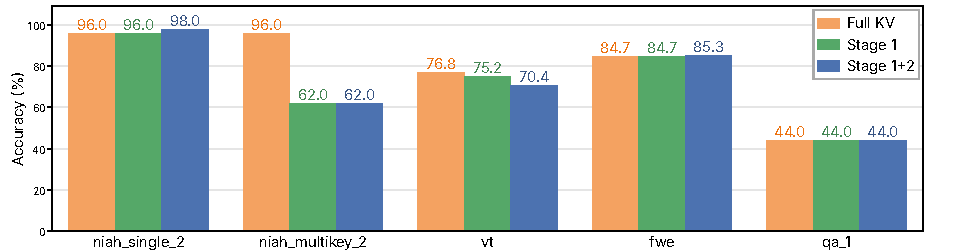
\includegraphics{figures/outputs/ruler-per-task.pdf}
\caption{\textbf{RULER accuracy per task with budget 1024, averaged over prompt lengths 2K to 32K} (10 samples per task and length). Stage~1+2 matches Full KV within a few points on four of the five tasks; the loss is concentrated in \code{niah\_multikey\_2}, which drops from 96.0 to 62.0, and Stage~1 alone loses the same amount there.}
\label{fig:per-task}
\end{figure}

\paragraph{Significance.}
We pair every method with Full KV on the same samples and bootstrap the mean difference (2000 resamples, stratified by task). Without the multi-key task, every configuration is within $\pm$1.2 points of Full KV and every 95\% confidence interval contains 0 (Table~\ref{tab:sig}). Doubling the budget to 2048 halves the multi-key loss.

\begin{table}[h]
\centering\small
\caption{Accuracy difference to Full KV (points) with 95\% bootstrap confidence intervals.}
\label{tab:sig}
\begin{tabular}{llllll}
\toprule
Config & Budget & RULER all & RULER w/o multi-key & RULER multi-key & LongBench \\
\midrule
E2 Stage 1 & 512 & $-8.4$ [$-11.2$, $-5.7$] & $-1.0$ [$-2.3$, $+0.2$] & $-38$ [$-50$, $-26$] & --- \\
E2 Stage 1 & 1024 & $-7.1$ [$-9.7$, $-4.5$] & $-0.4$ [$-1.4$, $+0.7$] & $-34$ [$-46$, $-22$] & $-0.9$ [$-2.2$, $+0.2$] \\
E2 Stage 1 & 2048 & $-3.7$ [$-5.8$, $-1.8$] & $-0.6$ [$-1.6$, $+0.3$] & $-16$ [$-26$, $-8$] & --- \\
E4 Stage 1+2 & 512 & $-7.7$ [$-10.6$, $-4.5$] & $-0.1$ [$-2.4$, $+2.3$] & $-38$ [$-50$, $-26$] & --- \\
E4 Stage 1+2 & 1024 & $-7.5$ [$-10.4$, $-4.5$] & $-0.9$ [$-3.0$, $+1.2$] & $-34$ [$-46$, $-22$] & $-1.4$ [$-2.9$, $-0.1$] \\
E4 Stage 1+2 & 2048 & $-4.2$ [$-6.6$, $-1.8$] & $-1.2$ [$-3.1$, $+0.6$] & $-16$ [$-26$, $-8$] & --- \\
\bottomrule
\end{tabular}
\end{table}

\paragraph{LongBench.}
On the more realistic LongBench (Table~\ref{tab:longbench}), a 1024-token budget over 32K inputs costs 1.3 points on average. Multi-document QA even improves slightly; the losses are in summarization, which needs the whole document, and in the synthetic retrieval tasks.

\begin{table}[h]
\centering\small
\caption{LongBench accuracy (\%), 16 tasks $\times$ 20 samples, 32K truncation, budget 1024.}
\label{tab:longbench}
\begin{tabular}{lrrrrrrr}
\toprule
Config & Single-doc QA & Multi-doc QA & Summ. & Few-shot & Synthetic & Code & Mean \\
\midrule
E0 Full KV & 42.9 & 33.7 & 27.6 & 69.9 & 45.0 & 53.5 & \best{44.9} \\
E2 Stage 1 & 43.0 & 35.0 & 25.3 & 70.0 & 40.0 & 52.6 & 44.1 ($-0.8$) \\
E4 Stage 1+2 & 40.9 & 35.0 & 25.9 & 68.7 & 40.0 & 52.9 & 43.6 ($-1.3$) \\
\bottomrule
\end{tabular}
\end{table}

\paragraph{Budget.}
Figure~\ref{fig:budget} sweeps the budget. At 16K, a budget of 4096 recovers Full KV accuracy; at 32K, accuracy stays near 69\% for all budgets because Stage~1's retained set grows only slowly with the budget.

\paragraph{Ablation: Stage~2 without eviction.}
E5 keeps the whole prompt and lets Stage~2 select from all of it; its chunk size and number of query dimensions follow from prompt length / budget (at 32K: chunk 6, $r = 24$, against chunk 3, $r = 68$ for E4, which selects from the $\sim$5.7K tokens Stage~1 retains; at 128K: chunk 12, $r = 12$). Up to 32K, E5 recovers almost all of the accuracy (Table~\ref{tab:ablation}): its mean is 1.1 points below Full KV with a confidence interval that contains 0, and multi-key retrieval returns from 62 to 98. This confirms that the RULER loss of E2/E4 comes from Stage~1's permanent eviction, not from Stage~2's sparse selection.

\begin{table}[h]
\centering\small
\caption{RULER accuracy (\%) with and without Stage~1 eviction, budget 1024, same samples (5 tasks $\times$ 10). $\Delta$: points vs Full KV with 95\% paired bootstrap CI.}
\label{tab:ablation}
\setlength{\tabcolsep}{4pt}
\begin{tabular}{lrrrrrrrl}
\toprule
Config & 2K & 4K & 8K & 16K & 32K & Mean & Multi-key & $\Delta$ vs Full KV \\
\midrule
E0 Full KV & 81.5 & 82.7 & 78.7 & 78.4 & 76.3 & \best{79.5} & 96.0 & --- \\
E4 Stage 1+2 & 75.1 & 78.0 & 69.9 & 67.6 & 69.2 & 71.9 & 62.0 & $-7.5$ [$-10.4$, $-4.5$] \\
E5 Stage 2 only & 81.5 & 80.4 & 75.2 & 77.9 & 76.9 & 78.4 & 98.0 & $-1.1$ [$-2.9$, $+0.8$] \\
\bottomrule
\end{tabular}
\end{table}

\paragraph{64K and 128K.}
With only 3 samples per task, these numbers are a coarse check: one sample moves a task score by 33 points, and no difference to Full KV is significant except E5's. Stage~1 and Stage~1+2 lose 4 points at 64K and 12--17 points at 128K, mostly in multi-key retrieval (Table~\ref{tab:long}). E5 is the best configuration at 64K but drops to 35.6 at 128K: at a compression ratio of 128, its chunks are 12 tokens long and it estimates scores from only 12 of 128 dimensions, too coarse to find the needle tokens (\code{fwe} 11 vs 56, \code{niah\_single\_2} 67 vs 100). Figure~\ref{fig:ruler-length} puts both experiments together: removing eviction helps up to 64K, while at 128K Stage~1 is needed to keep Stage~2's compression ratio moderate.

\begin{table}[h]
\centering\small
\caption{RULER accuracy (\%) at 64K and 128K, budget 1024, 5 tasks $\times$ 3 samples. $\Delta$: mean over both lengths vs Full KV, 95\% paired bootstrap CI.}
\label{tab:long}
\begin{tabular}{lrrrl}
\toprule
Config & 64K & 128K & Mean & $\Delta$ vs Full KV \\
\midrule
E0 Full KV & 69.3 & 67.1 & \best{68.2} & --- \\
E2 Stage 1 & 64.9 & 54.7 & 59.8 & $-8.4$ [$-19.8$, $+2.9$] \\
E4 Stage 1+2 & 65.8 & 49.8 & 57.8 & $-10.4$ [$-22.0$, $+0.7$] \\
E5 Stage 2 only & 71.1 & 35.6 & 53.3 & $-14.9$ [$-26.0$, $-4.2$] \\
\bottomrule
\end{tabular}
\end{table}

\begin{figure}[h]
\centering
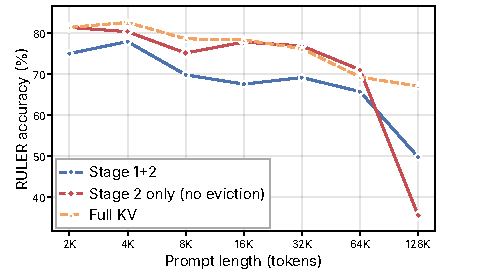
\includegraphics{figures/outputs/ruler-vs-length.pdf}
\caption{\textbf{RULER accuracy versus prompt length with budget 1024, with and without Stage~1 eviction.} Each point is the mean over 5 tasks, with 10 samples per task up to 32K and 3 at 64K and 128K; the x axis is logarithmic. Without eviction, Stage~2 alone stays close to Full KV up to 32K (mean 78.4 vs 79.5, against 71.9 for Stage~1+2), but at 128K it falls to 35.6, below both Full KV (67.1) and Stage~1+2 (49.8).}
\label{fig:ruler-length}
\end{figure}

\paragraph{CPU/Metal consistency.}
On 60 samples each at 2K/4K/8K, E1 vs E2 and E3 vs E4 produce \textbf{100\% identical} generations: the reordered floating-point reductions on Metal do not change a single output.

\begin{figure}[h]
\centering
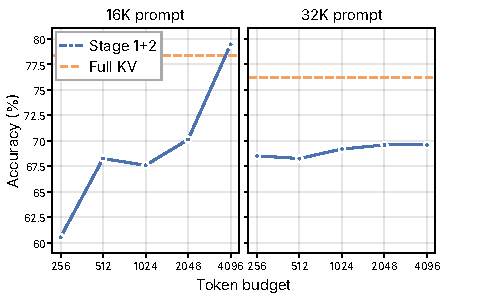
\includegraphics{figures/outputs/accuracy-vs-budget.pdf}
\caption{\textbf{RULER accuracy of Stage~1+2 versus token budget at 16K and 32K prompts}, averaged over five tasks. Budgets 512 to 2048 use 10 samples per task, 256 and 4096 use 5; the x axis is logarithmic and the dashed line marks Full KV. At 16K a budget of 4096 reaches Full KV (79.5 vs 78.4), while at 32K accuracy stays near 69 for every budget, 7 points below Full KV.}
\label{fig:budget}
\end{figure}

\subsection{Latency}

\paragraph{Decode latency.}
Table~\ref{tab:itl} and Figure~\ref{fig:itl} show the median inter-token latency (ITL). Full KV grows linearly with the context, because every step reads the whole KV cache. Stage~1+2 is nearly constant, because each step attends to a fixed number of selected tokens. Stage~1 alone sits in between: its retained set grows slowly (5643, 6250 and 6345 tokens at 32K, 64K and 128K). E2 is faster than Full KV from 8K on, and E4 from 32K on; at 128K the speedups are 3.15$\times$ and 2.91$\times$. Metal Stage~2 is 33--115$\times$ faster than the CPU reference.

\begin{table}[h]
\centering\small
\caption{Median decode latency (ms/token), budget 1024, 128 generated tokens. Speedup over Full KV in parentheses.}
\label{tab:itl}
\begin{tabular}{lrrrrrrr}
\toprule
Config & 2K & 4K & 8K & 16K & 32K & 64K & 128K \\
\midrule
E0 Full KV & 5.11 & 5.33 & 5.82 & 6.70 & 9.09 & 13.29 & 21.89 \\
E1 Stage 1 $\cdot$ CPU & 5.33 & 5.49 & 5.70 & 5.89 & 6.57 (1.38$\times$) & --- & --- \\
E2 Stage 1 $\cdot$ Metal & 5.33 & 5.48 & 5.69 (1.02$\times$) & 5.88 (1.14$\times$) & 6.55 (1.39$\times$) & 6.90 (1.93$\times$) & 6.96 (\best{3.15$\times$}) \\
E3 Stage 1+2 $\cdot$ CPU & 241 & 390 & 529 & 687 & 824 & --- & --- \\
E4 Stage 1+2 $\cdot$ Metal & 7.19 & 7.32 & 7.13 & 7.36 & 7.16 (1.27$\times$) & 7.44 (1.79$\times$) & 7.51 (\best{2.91$\times$}) \\
\bottomrule
\end{tabular}
\end{table}

\begin{figure}[h]
\centering
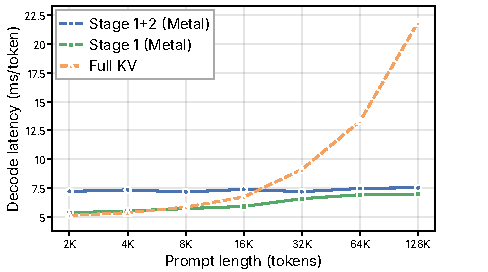
\includegraphics{figures/outputs/itl-vs-length.pdf}
\caption{\textbf{Per-token decode latency versus prompt length} (budget 1024). Each point is the median over 6 runs (3 at 64K and 128K); the x axis is logarithmic. Stage~1+2 stays between 7.13 and 7.51\,ms from 2K to 128K, while Full KV grows to 21.9\,ms, so at 128K Stage~1+2 is 2.91$\times$ faster.}
\label{fig:itl}
\end{figure}

E2 stays about 0.5\,ms faster than E4: attending to $\sim$6K retained tokens already costs less than Stage~2's fixed per-step selection overhead ($\sim$1.4\,ms). With this budget, Stage~2's value is not raw speed but that its attention cost is independent of the context length. The first E4 decode step is slower (10--24\,ms) because it builds the chunk summaries for all retained tokens.

\paragraph{Stage~2 without eviction.}
Stage~1 also matters for speed (Table~\ref{tab:ablation-latency}). Without eviction, E5's per-step cost grows with the context, because its scoring pass reads the summaries of every chunk of the whole prompt: 7.04\,ms at 2K but 11.98\,ms at 128K, against 7.50\,ms for E4. E5 is still 1.83$\times$ faster than Full KV at 128K, since it reads only chunk summaries and the selected tokens rather than the full KV cache, but it keeps the full KV cache in memory (14.3\,GB at 128K). E4 in this session reproduces the main benchmark within 0.1\,ms.

\begin{table}[h]
\centering\small
\caption{Decode latency (ms/token) with and without Stage~1 eviction, budget 1024, 128 generated tokens. E4 and E5 are interleaved in one session (3 runs per cell); Full KV is from Table~\ref{tab:itl}.}
\label{tab:ablation-latency}
\begin{tabular}{lrrrrrrr}
\toprule
Config & 2K & 4K & 8K & 16K & 32K & 64K & 128K \\
\midrule
E0 Full KV & 5.11 & 5.33 & 5.82 & 6.70 & 9.09 & 13.29 & 21.89 \\
E4 Stage 1+2 & 7.19 & 7.29 & 7.12 & 7.32 & 7.16 & 7.44 & \best{7.50} \\
E5 Stage 2 only & 7.04 & 7.09 & 7.32 & 7.38 & 7.97 & 9.81 & 11.98 \\
\bottomrule
\end{tabular}
\end{table}

\paragraph{Time to first token.}
TTFT is dominated by prefill (156\,ms at 2K, 8.9\,s at 32K, 109\,s at 128K), which RocketKV does not change. Stage~1 eviction takes 19--470\,ms on the CPU but 0.5--8.1\,ms on Metal (37--65$\times$ faster, $<$0.1\% of TTFT), so E2/E4 TTFT is within 1\% of Full KV.

\paragraph{Long generation.}
With 128 output tokens the end-to-end time is dominated by prefill, and all Metal configurations are within $\pm$4\% of Full KV. Longer outputs expose the decode savings (Figure~\ref{fig:long}): for 1024 tokens from a 32K prompt, total decode time is 9.40\,s (Full KV), 6.61\,s (E2, $-30\%$) and 7.41\,s (E4, $-21\%$); from a 128K prompt it is 22.46\,s, 7.05\,s ($-69\%$) and 7.54\,s ($-66\%$).

\begin{figure}[h]
\centering
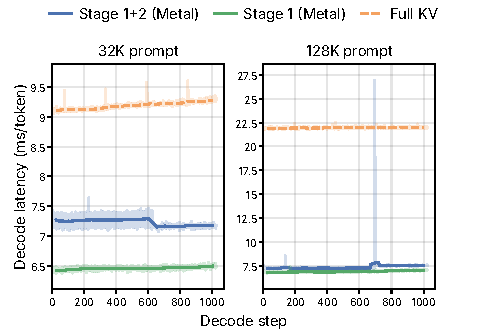
\includegraphics{figures/outputs/long-generation.pdf}
\caption{\textbf{Decode latency at each step of a 1024-token generation from a 32K and a 128K prompt} (budget 1024). Lines are smoothed with a moving average over 5\% of the steps; faint lines show raw values (median over 2 runs at 32K, 1 run at 128K). Full KV slows as the context grows, while both RocketKV variants stay flat; total decode time at 128K falls from 22.5\,s to 7.54\,s with Stage~1+2 ($-66\%$).}
\label{fig:long}
\end{figure}

\paragraph{Memory.}
Stage~1 shrinks the logical F16 KV cache from 878 to 389\,MB at 8K (2.3$\times$), 3519 to 617\,MB at 32K (5.7$\times$) and 14259 to 694\,MB at 128K (20.5$\times$). Peak RSS does not drop, because \code{llama.cpp} pre-allocates the KV buffer for \code{n\_ctx}; turning the logical saving into real memory needs compaction or re-allocation after eviction.

\subsection{Discussion and limitations}
\begin{itemize}
\item \textbf{When RocketKV is faster.} The 3B model's weights are $\sim$3.4\,GB, so short-context decode is bound by weight reads. KV reads grow with the context and match the weights at $\sim$32K, which is where RocketKV starts to pay off.
\item \textbf{Accuracy cost is in Stage~1, but Stage~1 is needed at 128K.} Multi-key retrieval is sensitive to permanent eviction; a larger budget, or Stage~2 alone without eviction (E5), recovers it up to 64K. At 128K, however, Stage~2 alone has to compress by 128$\times$ and its approximate scores become too coarse, so the two stages are complementary: Stage~1 keeps Stage~2's compression ratio moderate.
\item \textbf{A bug found by the benchmark.} The first run failed at RULER 2K, budget 2048: when $\lceil k/64\rceil \cdot 60 \ge k$, \code{attend} produced empty blocks and NaN on merge. The runner's finiteness check turned this into an error rather than a silent wrong result; all experiments were re-run after the fix. Kernel tests should cover split boundaries, not only random shapes.
\item \textbf{Limitations.} 64K/128K accuracy uses only 3 samples per task, so it is a coarse check; one 3B model on one machine; RULER uses 5 of 13 tasks with 10 samples each and LongBench 20 samples per task, so per-task errors are several points; the memory saving is not realized in process memory; Stage~2 requires patching \code{llama.cpp}.
\end{itemize}

\section{Conclusion}
RocketKV on Metal makes long-context decode on Apple silicon faster than Full KV, and the gap grows with the context: 1.39$\times$/1.27$\times$ (Stage~1 / Stage~1+2) at 32K and 3.15$\times$/2.91$\times$ at 128K, with Stage~1+2 decode nearly constant at 7.1--7.5\,ms/token. The Metal kernels are essential: they make Stage~2 33--115$\times$ faster than the CPU reference while producing identical outputs. The price is a 1.3-point drop on LongBench and a 7.6-point drop on RULER that comes almost entirely from multi-key retrieval and can be bought back with a larger budget. The ablation shows that this loss is caused by Stage~1's eviction: Stage~2 alone matches Full KV up to 32K. Stage~1 is still worth its cost at long contexts: it keeps Stage~2's compression ratio moderate (Stage~2 alone drops to 35.6 at 128K, against 49.8 with both stages) and keeps decode time flat (7.50 vs 11.98\,ms/token at 128K).

\end{document}
